\documentclass[10pt,a4paper]{article}
\usepackage[margin=2cm]{geometry}
\usepackage{mathtools}
\usepackage{enumerate}
\usepackage{float}
\usepackage{graphicx}
\usepackage{amssymb}
\usepackage[utf8]{inputenc}
\usepackage{listings}
\usepackage{amsthm}
\usepackage{color}
\usepackage{tikz}

\begin{document}
\section*{Descriptive statistics}
\begin{table}[!htbp] \centering 
  \caption{Descriptive statistics (\$)} 
  \label{} 
\begin{tabular}{@{\extracolsep{5pt}}lcccccccc} 
\\[-1.8ex]\hline 
\hline \\[-1.8ex] 
Statistic & \multicolumn{1}{c}{N} & \multicolumn{1}{c}{Mean} & \multicolumn{1}{c}{St. Dev.} & \multicolumn{1}{c}{Min} & \multicolumn{1}{c}{Pctl(25)} & \multicolumn{1}{c}{Median} & \multicolumn{1}{c}{Pctl(75)} & \multicolumn{1}{c}{Max} \\ 
\hline \\[-1.8ex] 
car & 20,623 & 154,052.700 & 129,354.400 & $-$5,300 & 74,800 & 120,400 & 190,000 & 1,408,000 \\ 
alternative transit & 5,734 & 157,011.300 & 130,547.500 & $-$5,300 & 72,000 & 124,650 & 200,000 & 1,365,000 \\ 
bus & 1,474 & 134,334.000 & 113,033.700 & $-$5,300 & 57,075 & 107,250 & 178,750 & 1,015,000 \\ 
street car & 117 & 191,273.800 & 149,999.500 & 14,000 & 95,000 & 147,960 & 245,000 & 618,000 \\ 
subway & 1,397 & 162,366.200 & 128,105.100 & 4,300 & 82,000 & 130,000 & 200,600 & 1,365,000 \\ 
rail & 390 & 184,171.700 & 140,021.900 & 870 & 89,350 & 148,500 & 224,500 & 920,000 \\ 
bike & 624 & 151,124.300 & 136,148.800 & $-$5,300 & 65,675 & 117,000 & 186,450 & 1,332,704 \\ 
home & 1,732 & 165,682.100 & 137,687.200 & $-$4,000 & 73,750 & 130,150 & 207,025 & 1,004,000 \\
\hline \\[-1.8 ex]
everyone & 26,357 & 154,696.300 & 129,618.100 & \$-\$5,300 & 74,000 & 121,200 & 191,000 & 1,408,000 \\
\hline \\[-1.8ex] 
\end{tabular} 
\end{table}

\section*{boxplot}
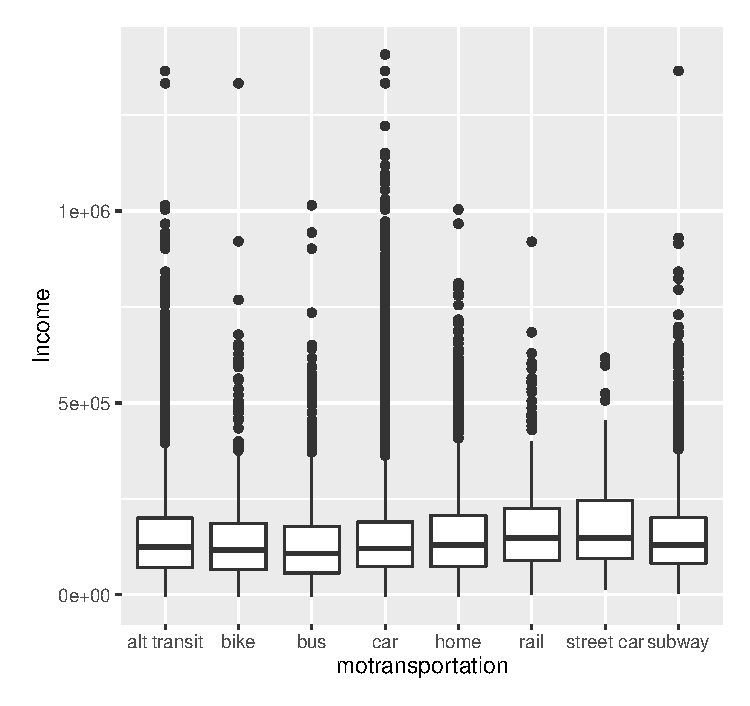
\includegraphics{Rplot.eps}
\newpage
\section*{Regression}
% Table created by stargazer v.5.2 by Marek Hlavac, Harvard University. E-mail: hlavac at fas.harvard.edu
% Date and time: Thu, Apr 28, 2016 - 13:43:17
\begin{table}[!htbp] \centering 
  \caption{Basic Regression alternate transit on log(HINC)} 
  \label{} 
\begin{tabular}{@{\extracolsep{5pt}}lc} 
\\[-1.8ex]\hline 
\hline \\[-1.8ex] 
 & \multicolumn{1}{c}{\textit{Dependent variable:}} \\ 
\cline{2-2} 
\\[-1.8ex] & atransit \\ 
\hline \\[-1.8ex] 
 logincome & 0.0001 \\ 
  & (0.003) \\ 
  & \\ 
 Constant & 0.205$^{***}$ \\ 
  & (0.035) \\ 
  & \\ 
\hline \\[-1.8ex] 
Observations & 27,708 \\ 
Log Likelihood & $-$14,275.070 \\ 
Akaike Inf. Crit. & 28,554.140 \\ 
\hline 
\hline \\[-1.8ex] 
\textit{Note:}  & \multicolumn{1}{r}{$^{*}$p$<$0.1; $^{**}$p$<$0.05; $^{***}$p$<$0.01} \\ 
\end{tabular} 
\end{table} 

\end{document}